
\de{ĐỀ THI HỌC KỲ I NĂM HỌC 2022-2023}{THPT Nguyễn Chí Thanh}


\begin{bt}%[0T2B1-1]%[0T3B1-2]%[0T3B2-3]%[Dự án đề kiểm tra HKI NH22-23 - Quang Anh]%[Nguyễn Chí Thanh]
	\begin{enumerate}
	\item Biểu diễn miền nghiệm của bất phương trình $x+2y-8 \leq 0$ trên mặt phẳng toạ độ $Oxy$.
	\item Tìm tập xác định của hàm số $y=f(x)=\dfrac{\sqrt{4-x}+\sqrt{x+2}}{x^{2}-5x+6}$.
	\item Vẽ đồ thị hàm số $(P)\colon y=x^{2}-2x+2$.
	\end{enumerate}
	\loigiai{\begin{enumerate}
			\immini{\item Vẽ đường thẳng $ d\colon y=-\dfrac{1}{2}x+4 $.\\
				Đường thẳng đi qua hai điểm $(0; 4)$ và $(2; 3)$.\\
				Xét điểm $O(0; 0)$ không thuộc đường thẳng $ d $, ta có $ 0+2\cdot 0-8\le 0 $ là mệnh đề đúng.\\
				Vậy miền nghiệm của bất phương trình $ x+2y-8\le 0 $ là phần không bị gạch sọc hình vẽ bên, chứa điểm $ O $ và kể cả đường thẳng $ d $.}{
				\begin{tikzpicture}[scale=0.8, font=\footnotesize, line join=round, line cap=round,>=stealth]
					\begin{scope}
						\clip (-1,-1) rectangle (9,5); 
						\fill[opacity=.2,pattern=north west lines] (-3,5.5)--(11,5.5)--(11,-1.5)--cycle; 
						\draw (-2,5)--(10,-1) node[midway,above,sloped]{$d$}; 
					\end{scope}
					\foreach\y in{1,2,3,4} 
					\draw (1pt,\y)--(-1pt,\y) node[left]{$\y$}; 
					\foreach\x in {1,2,3,4,5,6,7,8} 
					\draw (\x,1pt)--(\x,-1pt) node[below]{$\x$}; 
					\draw[dashed] (2,0)--(2,3)--(0,3); 
					\draw[->] (-1,0)--(9,0) node[below]{$x$}; 
					\draw[->] (0,-1)--(0,5) node[left]{$y$}; 
					\draw (0,0) node[below left]{$O$}; 
				\end{tikzpicture}
			}
			\item 	Điều kiện xác định của hàm số
			$$\heva{&4-x\ge 0\\&x+2\ge 0\\&x^2-5x+6\ne 0}\Leftrightarrow\heva{&x\le 4\\&x\ge-2\\&x\ne 2\\&x\ne 3}\Leftrightarrow\heva{&-2\le x\le 4\\&x\ne 2\\&x\ne 3.}$$ 
			Tập xác định của hàm số là $\mathscr{D}=[-2; 4]\setminus\{2; 3\}$.
			\immini{\item Đồ thị hàm số có trục đối xứng $ x=1 $.\\
				Đỉnh $ I(1; 1)$.\\
				Bảng giá trị của hàm số 
				\begin{center}
					\begin{tabular}{|c|c|c|c|c|c|}
						\hline
						$ x $ & $-1 $ & $ 0 $ & $ 1 $ & $ 2 $ & $ 3 $\\
						\hline
						$ y $ & $ 5 $ & $ 2 $ & $ 1 $ & $ 2 $ & $ 5 $\\
						\hline
					\end{tabular}
			\end{center}}
			{
				\begin{tikzpicture}[scale=1, font=\footnotesize, line join=round, line cap=round,>=stealth]
					\begin{scope}[yscale=.8]
						\draw[->] (-2.1,0)--(4.1,0) node[below left] {$x$}; 
						\draw[->] (0,-1.1)--(0,6.1) node[below left] {$y$}; 
						\draw (0,0) node [below left] {$O$}; 
						\foreach\x in {-1,1,2,3}
						\draw[thin] (\x,1pt)--(\x,-1pt) node [below] {$\x$}; 
						\foreach\y in {5,2,1}
						\draw[thin] (1pt,\y)--(-1pt,\y) node [below left] {$\y$}; 
						\draw[dashed,thin](1,0)--(1,1)--(0,1); 
						\draw[dashed,thin](2,0)--(2,2)--(0,2); 
						\draw[dashed,thin](3,0)--(3,5)--(0,5); 
						\draw[dashed,thin](-1,0)--(-1,5)--(0,5); 
						\begin{scope}
							\clip (-2,-1) rectangle (4,6); 
							\draw[samples=200,domain=-2:4,smooth,variable=\x] plot (\x,{1*(\x)^2+-2*(\x)+2}); 
						\end{scope}
					\end{scope}
				\end{tikzpicture}
			}
		\end{enumerate}
	
	}
\end{bt}

\begin{bt}%[0T6B4-2]%[Dự án đề kiểm tra HKI NH22-23 - Quang Anh]%[Nguyễn Chí Thanh]
	Sản lượng lúa (tạ) của $ 40 $ thửa ruộng thí nghiệm có cùng diện tích được trình bày trong bảng tần số sau
	\begin{center}
		\begin{tabular}{|c|c|c|c|c|c|c|}
			\hline
			Sản lượng ($ x $) & $ 20 $ & $ 21 $ & $ 22 $ & $ 23 $ & $ 24 $ &\\
			\hline
			Tần số ($ n $) & $ 5 $ & $ 8 $ & $ 11 $ & $ 10 $ & $ 6 $ & $ N=40 $\\
			\hline
		\end{tabular}
	\end{center}
	Tìm năng suất lúa trung bình, tứ phân vị, mốt và phương sai của bảng số liệu trên.
	\loigiai{
		\begin{itemize}
			\item Năng suất lúa trung bình 
			$$\overline{x}=\dfrac{20\cdot 5+21\cdot 8+22\cdot 11+23\cdot 10+24\cdot 6}{40}=22{,}1. $$ 
			\item Vì cỡ mẫu $ N=40 $, nên giá trị tứ phân vị thứ hai là $ Q_2=\dfrac{1}{2}(22+22)=22 $.\\
			Tứ phân vị thứ nhất là $ Q_1=\dfrac{1}{2}(21+21)=21 $.\\
			Tứ phân vị thứ ba là $ Q_3=\dfrac{1}{2}(23+23)=23 $.
			\item Sản lượng lúa $ 22 $ tạ đạt được tại $ 11 $ thửa ruộng. Do đó mẫu số liệu trên có $ M_0=22 $.\\
			\item Phương sai của mẫu số liệu này là
			\allowdisplaybreaks
			\begin{eqnarray*}
				S^2&=&\dfrac{1}{40}\left[5(20-22{,}1)^2+8(21-22{,}1)^2+11(22-22{,}1)^2+10(23-22{,}1)^2+6(24-22{,}1)^2\right]\\
				&=&1{,}54.
			\end{eqnarray*}
		\end{itemize}
	}
\end{bt}
\begin{bt}%[0T4B3-1]%[0T4B2-1]%[Dự án đề kiểm tra HKI NH22-23 - Quang Anh]%[Nguyễn Chí Thanh]
		\begin{enumerate}
		\immini{\item Trên biển một con thuyền thả neo ở vị trí $ A $. Một người đứng ở vị trí $ K $ trên bờ biển muốn đo khoảng cách từ người đó đến con thuyền, người đó đã chọn một điểm $ H $ trên bờ với $ K $ và đo được $ KH=380 $ m, $\widehat{AKH}=50^\circ $, $\widehat{AHK}=45^\circ $. Khoảng cách $ KA $ từ người đó đến con thuyền bằng bao nhiêu? (làm tròn đến hàng đơn vị)}{
			\begin{tikzpicture}[scale=1, font=\footnotesize, line join=round, line cap=round,>=stealth]
				\tikzset{thuyen/.pic={
						\begin{scope}[scale=.1]
							\fill[red](-0.36,3.8)--++(180:2)--(-0.36,4.5)--cycle; 
							\draw[orange,line width=2pt](-0.4,-3.2)--++(90:7.8); 
							\fill[ball color=orange!60!black](-3.9,-4.35)--(2.75,-4.35)--++(43:1.4)--++(182:8.1)--cycle; 
							\fill[ball color=yellow](-4.5,-3.55)--++(1.8:8.75)--++(65:0.7)--++(184.2:9.1)--cycle; 
							\fill(-4.2,-3.3)..controls++(45:2.5) and ++(-108:3)..(-0.45,2.7)..controls++(-95:2) and ++(100:2)..(-0.45,-2.6); 
							\fill[ball color=teal!50!green](-0.4,-2.6)..controls++(20:1) and ++(160:2)..(3.75,-2.7)..controls++(105:3.25) and ++(-35:2)..(-0.4,3.65)..controls++(-65:2) and ++(65:2)..(-0.4,-2.6); 
						\end{scope}
				}}
				\path (0,0) coordinate (A) 
				(A)+(90:.5) pic{thuyen}
				(-2,-2) coordinate (H)
				(2,-1.5) coordinate (K)
				; 
				\foreach\i/\g in {K/-90, H/-90, A/-90}
				\fill (\i) circle (1.5pt)+(\g:3mm) node {$\i$}; 
				\draw (H)--(A)--(K)--cycle; 
				\node at ($(H)!.5!(K)$) [below]{$380 $ m}; 
				\draw pic[" $ 45^\circ $ ", draw=black, angle eccentricity=1.5, angle radius=.5cm]
				{angle=K--H--A}; %góc
				\draw pic[" $ 50^\circ $ ", draw=black, angle eccentricity=1.5, angle radius=.5cm]
				{angle=A--K--H}; %góc
			\end{tikzpicture}
		}
		\item Cho tam giác $A B C$ có cạnh $a=2 \sqrt{3} \mathrm{~cm}$, $b=2 \mathrm{~cm}$ và $\widehat{C}=30^{\circ}$. Tính diện tích tam giác $A B C$, bán kính đường tròn ngoại tiếp và nội tiếp tam giác $\mathrm{ABC}$.
	\end{enumerate}
	\loigiai{
		\begin{enumerate}
			\item Ta có $\widehat{HAK}=180^\circ-\widehat{AHK}-\widehat{AKH}=180^\circ-45^\circ-50^\circ=85^\circ $.\\
			Áp dụng định lý sin cho tam giác $ AHK $, ta có
			$$\dfrac{AK}{\sin\widehat{AHK}}=\dfrac{HK}{\sin\widehat{HAK}}\Leftrightarrow\dfrac{AK}{\sin 45^\circ}=\dfrac{380}{\sin 85^\circ}\Leftrightarrow AK\approx 270 \text{ m}. $$ 
			\item Diện tích tam giác $ ABC $ là $ S=\dfrac{1}{2}\cdot a\cdot b\cdot\sin C=\dfrac{1}{2}\cdot 2\sqrt{3}\cdot 2\cdot\sin 30^\circ=\sqrt{3}$ (cm$^2$).\\
			Ta có $ c^2=a^2+b^2-2ab\cdot\cos C=(2\sqrt{3})^2+2^2-2\cdot 2\sqrt{3}\cdot 2\cdot\cos 30^\circ=4 $, suy ra $ c=2 $.\\
			Bán kính đường tròn ngoại tiếp là $ 2R=\dfrac{c}{\sin C}\Leftrightarrow R=\dfrac{2}{2\sin 30^\circ}=2 $ (cm).\\
			Nửa chi vi tam giác là $ p=\dfrac{2\sqrt{3}+2+2}{2}=2+\sqrt{3}$ (cm).\\
			Bán kính đường tròn nội tiếp tam giác là $ r=\dfrac{S}{p}=\dfrac{\sqrt{3}}{2+\sqrt{3}}=-3+2\sqrt{3}$ (cm).
		\end{enumerate}
	}
\end{bt}


\begin{bt}%[0T5K3-2]%[Dự án đề kiểm tra HKI NH22-23- Phạm Phương]%[TRƯỜNG THPT NGUYỄN CHÍ THANH]
\begin{enumerate}
\item Cho tứ giác $ABCD$. Gọi $P$, $Q$ lần lượt là trung điểm của $AD$, $BC$. Chứng minh\break $\overrightarrow{AB}-\overrightarrow{CD}=2 \overrightarrow{PQ}$.
\item Cho ba lực $\vec{F_1}=\overrightarrow{MA}$, $\vec{F_2}=\overrightarrow{MB}$ và $\vec{F_3}=\overrightarrow{MC}$ cùng tác động vào một vật tại điểm $M$ và vật đứng yên. Cho biết độ lớn của $\vec{F_1}$, $\vec{F_2}$ đều là $200$ N và $\widehat{AMB}=60^{\circ}$. Tìm độ lớn của lực $\vec{F_3}$.
\end{enumerate}
%\dapso{b) $\left| \vec{F}_{3}\right| =200 \sqrt{3}\mathrm{~N}$.}
\loigiai{
\begin{enumerate}
	\immini{
	\item $P$ là trung điểm $AD$ suy ra $2\vec{AP}=\vec{AD}$;\\
	$Q$ là trung điểm $BC$ suy ra $\vec{AB}+\vec{AC}=2\vec{AQ}$.\\
	Ta có 
	\allowdisplaybreaks\begin{eqnarray*}
		\vec{AB}-\vec{CD}&= &\vec{AB}-\vec{AD}+\vec{AC} \\
		&= & 2\vec{AQ}-2\vec{AP} \\
		&= & 2\vec{PQ} \text{ (điều phải chứng minh)}.
	\end{eqnarray*}
}{
\begin{tikzpicture}[scale=1,>=stealth, font=\footnotesize, line join=round, line cap=round]
	\foreach \i/\j/\k in{0/0/A,-1/-2/B,3/-2.5/C,4.3/0.7/D}
	\coordinate (\k) at(\i,\j);
	\draw (A)--(B)--(C)--(D)--cycle;
	\coordinate (P) at ($(A)!0.5!(D)$);
	\coordinate (Q) at ($(B)!0.5!(C)$);
	\foreach \p/\r in {A/135,B/-135,C/-45,D/45,P/90,Q/-90}
	\fill (\p) circle (1pt) node[shift={(\r:3mm)}]{$\p$};
	\node at ($(A)!0.5!(P)$){|};
	\node at ($(D)!0.5!(P)$){|};
	\node at ($(B)!0.5!(Q)$)[rotate=-10]{$\parallel$};
	\node at ($(C)!0.5!(Q)$)[rotate=-10]{$\parallel$};
\end{tikzpicture}
}
	\item Do vật đứng yên nên $\vec{F_1}+\vec{F_2}+\vec{F_3}=\vec{0}$.\\
	Gọi $D$ là đỉnh thứ $4$ của hình bình hành $MADB$.
	\begin{center}
		\begin{tikzpicture}[scale=1, font=\footnotesize, line join=round, line cap=round, >=stealth]
			\path 
			(0,0) coordinate (M)
			+(-20:3) coordinate (B)
			+(40:3) coordinate (A)
			($(A)+(B)-(M)$) coordinate (D)
			($(D)!2!(M)$) coordinate (C)
			($(A)!.5!(B)$) coordinate (I);			
			\draw[->] (M)--(A) node[midway,above,sloped] {$\vec{F_1}$};
			\draw[->] (M)--(B) node[midway,below,sloped] {$\vec{F_2}$};
			\draw[->] (M)--(D) node[midway,above left,sloped] {$\vec{F_1}+\vec{F_2}$};
			\draw[->] (M)--(C) node[midway,above,sloped] {$\vec{F_3}$};
			\draw (A)--(B) (A)--(D)--(B);			
			\foreach \p/\r in {A/90,B/-20,M/135,C/135,D/45,I/-20}
			\fill (\p) circle (1.5pt) node[shift={(\r:3mm)}]{$\p$};
		\end{tikzpicture}
	\end{center}
	Khi đó $\vec{F_3}=-(\vec{F_1}+\vec{F_2})=-(\vec{MA}+\vec{MB})=-\vec{MD}$.\\
	Do đó, $\vec{F_3}$ ngược hướng với $\vec{MD}$ và có độ lớn bằng $\vec{MD}$.
	Gọi $I$ là giao điểm của $AB$ và $CD$.  Khi đó $I$ là trung điểm của $AB$ và $MD$.\\
	Mà $\widehat{AMB}=60^\circ$ nên tam giác $AMB$ đều.\\
	Suy ra $MI=MA\cdot \dfrac{\sqrt{3}}{2}=200\cdot \dfrac{\sqrt{3}}{2}=100\sqrt{3}$.\\
	Vậy độ lớn của lực $\vec{F_3}$ là $\left|\vec{F_3}\right|=MD=2MI=200\sqrt{3}$ (N).
\end{enumerate}
}
\end{bt}
%----Câu 5
\begin{bt}%[0T2G2-2]%[Dự án đề kiểm tra HKI NH22-23- Phạm Phương]%[TRƯỜNG THPT NGUYỄN CHÍ THANH]
Một phân xưởng cần sản xuất ra hai loại sản phẩm. Để sản xuất $1$ kilogam sản phẩm loại I cần sử dụng máy trong 20 giờ và tiêu tốn $2$ kilogam nguyên liệu. Để sản xuất $1$ kilogam sản phẩm loại II cần sử dụng máy trong $10$ giờ và tốn 3 kilogam nguyên liệu. Biết rằng 1 kilogam sản phẩm loại I thu lãi được $50\,000$ đồng, $1$ kilogam sản phẩm Ioại II thu lãi được $40\,000$ đồng, có thể sử dụng máy tối đa $1\,200$ giờ và có $300$ kilogam nguyên liệu. Hỏi phân xưởng đó nên sản xuất mỗi loại sản phẩm bao nhiêu kilogam để thu lãi cao nhất?
%\dapso{Loại I: $15$ kg; Loại II: $90$ kg}
\loigiai{
\immini{Gọi $x$, $y$ ($x$, $y\in \mathbb{N}$) lần lượt là số kilogam sản phẩm loại I, II. Ta có hệ bất phương trình
	$$\heva{&x\ge 0\\&y\ge 0\\&20x+10y\le 1\,200\\&2x+3y\le 300.}$$
	Biểu diễn miền nghiệm của hệ bất phương trình trên hệ trục tọa độ $Oxy$, ta được hình vẽ bên.\\
	Miền nghiệm là miền tứ giác $OABC$ với các đỉnh $O(0;0)$, $A(60;0)$, $B(15;90)$, $C(0;100)$.\\
	Gọi $L$ là số tiền lãi thu được, ta có $$L=50\,000x+40\,000y.$$
	Bảng giá trị của $L$ tại các đỉnh của tứ giác}{
	\begin{tikzpicture}[scale=1, font=\footnotesize, line join=round, line cap=round, >=stealth]
		\begin{scope}[yscale=.6,xscale=.5]
			\draw[->] (-1,0)--(13,0) node[below]{$x$};
			\draw[->] (0,-1)--(0,14) node[right]{$y$};
			\begin{scope}
				\clip (-1,-1) rectangle (13,14);
				\fill[opacity=.5,pattern=north east lines] (-3,18)--(14,18)--(14,-16)--cycle;
				\fill[opacity=.5,pattern=north west lines] (-1,0)--(-1,-1)--(13,-1)--(13,0)--cycle;
				\fill[opacity=.5,pattern=north east lines] (-10,16.67)--(17,16.67)--(17,-1.33)--cycle;
				\fill[opacity=.5,pattern=north west lines] (-1,-1)--(0,-1)--(0,16)--(-1,16)--cycle;
				\draw (-2,16)--(6.5,-1);
				\draw (-9,16)--(16.5,-1);
			\end{scope}
			\draw[fill=black] (6,0) circle (1pt) node[above left]{$A$} (0,0) circle (1pt) node [below left] {$O$} (1.5,9) circle (1pt) node[below left]{$B$} (0,10) circle (1pt) node[right]{$C$};
			\draw (6,1pt)--(6,-1pt) node[below left]{$60$} (1.5,1pt)--(1.5,-1pt) node[below]{$15$};
			\draw (1pt,10)--(-1pt,10) node[left]{$100$} (1pt,9)--(-1pt,9) node[left]{$90$} (1pt,12)--(-1pt,12) node[left]{$120$};
			\draw[dashed] (1.5,0)--(1.5,9)--(0,9);
		\end{scope}
	\end{tikzpicture}
}
\begin{center}
	\begin{tabular}{|c|c|c|c|c|}
		\hline
		& $O(0;0)$ & $A(60;0)$ & $B(15;90)$ & $C(0;100)$\\
		\hline
		$L=50\,000x+40\,000y$& $0$ & $3\,000\,000$ & $4\,350\,000$ & $4\,000\,000$\\
		\hline
	\end{tabular}
\end{center}
Dựa vào bảng, $L$ đạt giá trị lớn nhất bằng $4\,350\,000$ tại $B(15;90)$.\\
Vậy phân xưởng đó nên sản xuất $15$ kilogam sản phẩm loại I và $90$ kilogam sản phẩm loại II để thu lãi cao nhất.
}
\end{bt}
%----Câu 6
\begin{bt}%[0T3G2-5]%[Dự án đề kiểm tra HKI NH22-23- Phạm Phương]%[TRƯỜNG THPT NGUYỄN CHÍ THANH]
\immini[thm]{Khi một quả bóng được đá lên, nó sẽ bay theo quỹ đạo của một cung parabol trong mặt phẳng tọa độ $Oth$ như hình bên, trong đó $t$ là thời gian kể từ khi quả bóng được đá lên (tính bằng giây), $h$ là độ cao (tính bằng mét) của quả bóng. Giả sử quả bóng được đá lên từ độ cao $1{,}1$ m. Sau $1$ giây nó đạt độ cao $8{,}6$ m. Sau 2 giây, nó đạt độ cao $6$ m. Hỏi độ cao lớn nhất mà quả bóng đạt được là bao nhiêu? (làm tròn đến hàng phần chục).
}{
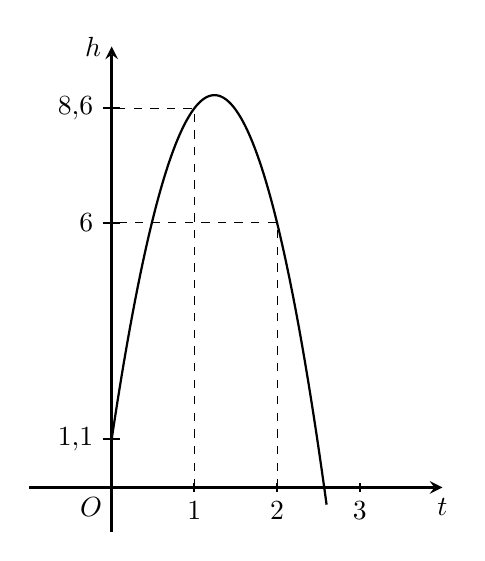
\begin{tikzpicture}[>=stealth,x=1.5cm,y=0.8cm,scale=0.7, font=\normalsize]
\def\a{-5.05} 
\def\b{12.55}
\def\c{1.1}
\draw[line width=1,->] (-1,0) -- (4,0) node[below] {$t$};
\draw[line width=1,->] (0,-1) -- (0,10) node[left] {$h$};
\draw (0,0)node[below left]{$O$};
\draw[thick,samples=150,smooth,domain=0:2.6] plot(\x,{\a*(\x)^2+(\b)*\x+(\c)}) ;
\foreach \x in {1,2,3} \draw[line width=0.75] (\x,0.1)--(\x,-0.1) node [below] {$\x$} ;
\foreach \y/\nhan in {1.1/1{,}1,8.6/8{,}6,6/6}\draw[line width=0.75] (0.1,\y)--(-0.1,\y) node [left] {$\nhan$}; 
\draw[dashed] (1,0)|-(0,8.6) (2,0)|-(0,6);
\end{tikzpicture}}
%\dapso{$8{,}90$ m}
\loigiai{
Quỹ đạo của quả bóng có phương trình $h(t)=at^2+bt+c$.\\
Ta có hệ phương trình sau
$$\heva{&h(0)=1{,}1\\&h(1)=8{,}6\\&h(2)=6}
\Leftrightarrow\heva{&c=1{,}1\\&a+b+c=8{,}6\\&4a+2b+c=6}
\Leftrightarrow  \heva{&a=-5{,}05\\&b=12{,}55\\&c=1{,}1.}\Rightarrow h(t)=-5{,}05t^2+12{,}55t+1{,}1.$$\\
Vậy độ cao lớn nhất quả bóng đạt được tại đỉnh parabol. Gọi $S$ là đỉnh của parabol ta có
\begin{itemize}
	\item $x_S=\dfrac{-12{,}55}{2\cdot (-5{,}05)}=\dfrac{251}{202}$.
	\item $y_S=h\left(\dfrac{251}{202}\right)=-5{,}05\cdot \left(\dfrac{251}{202}\right)^2+12{,}55\cdot \left(\dfrac{251}{202}\right)+1{,}1 \approx 8{,}9$.
\end{itemize}
Vậy độ cao lớn nhất mà quả bóng đạt được khoảng $8{,}9$ m.
}
\end{bt} 





